\documentclass{article}
\usepackage{graphicx}
\usepackage{cite}
\usepackage[lined,ruled,vlined,linesnumbered]{algorithm2e}
\usepackage{fixltx2e}
\usepackage{float}
\setlength{\parskip}{1em}
\graphicspath{ {images/} }

\title{Fuzzy Based Rule System}
\author{Grant Christie}
\date{}

\begin{document}
\maketitle

\section{Fuzzy Logic Overview}
Fuzzy Logic is a form of many-valued logic where the truth values of variables may be any real number between 1 and 0 as opposed to Boolean Logic where the values may only be 1 or 0. This method of reasoning is more akin to the way humans make decisions as they consider all the possibilities in between the traditional digital values YES and NO. The architecture of a Fuzzy Logic System has four main parts:

\begin{itemize}
  \item Fuzzifier - This transforms the system’s inputs into fuzzy sets.
  \item Knowledge Base - This stores the IF THEN rules provided by experts.
  \item Inference Engine - This performs the reasoning process by making fuzzy inference on the inputs and IF THEN rules.
  \item Defuzzifier - This transforms the fuzzy set acquired from the inference engine into a crisp value.
\end{itemize}

\begin{figure}[H]
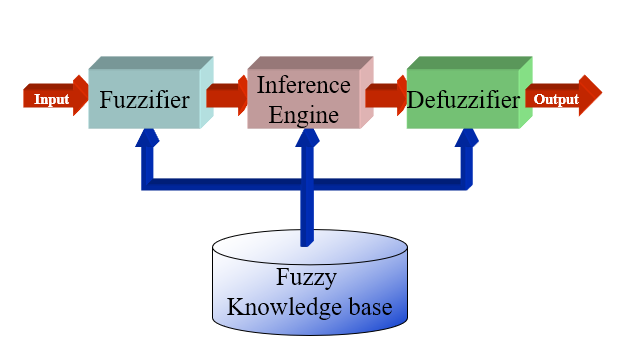
\includegraphics[width=12cm]{architecture}
\caption{Fuzzy Logic System Architecture}
\end{figure}

As shown above, the Fuzzifier turns a crisp input into a fuzzy set, a fuzzy set is simply a set which has a fuzzy boundary. For example, if we have a set 'A' of young people, in a crisp set an element either belongs in the set A or does not belong in the set A. Therefore, there needs to be a value in which anything below that number is classed as young and anything above that number is classed as old, say 40. However, in the real world it may seem odd to classify a 39 year old and a 5 year old in the same manner, this is where fuzzy sets help. Fuzzy logic makes use of membership functions to determine how much a given value belongs to a set. Membership functions map each element to a value between 1 and 0 which quantifies the degree of membership of the element in the fuzzy set. An important thing to note is that membership functions are subjective measures so different systems may provide different results depending on their implementation. Therefore, in this example we give 40 the value 0.5, this represents the middle point of young and not young. A person who is age 1 is likely to have the value 1 as they are definitely young, however a person aged 20 may have the value 0.75 as they are starting to become older and now belong less to the set A. As can be seen if the 0.5 value had been set at a different age, say 30, the membership value of the 20 year old would not be the same.

Once the system has used the membership functions to convert the crisp data into a fuzzy set the rule base within the inference engine is then used to evaluate the rules. Each rule must be examined and for each rule, the likelihood that that rule will be executed is calculated. To determine this the main part of the rule that must be looked at is the logical operator, AND or OR. If the AND operator is used, then the minimum value must be used and if the OR operator is being used then the maximum value must be used. After each rule has been examined and a value or values have been obtained for each, the system must then combine the results to have a single value for each one. As each of the rules in the rule base are to be treated independently from one another the system uses OR which again equates to finding the MAX of the given values.

Finally, the system uses these fuzzy values to perform defuzzification. To do this the system will use the following equation:
\[ 
	x = \frac {\sum A_i X_i}{\sum A_i}
\]
Where,
A\textsubscript{i}= areas of the membership regions.
X\textsubscript{i} = centres of the membership regions.

To calculate the area of the membership regions the system must multiply the length of the base of the curve by the relevant fuzzy values and then multiply the result of that by 0.5. The centre is simply the halfway point of the membership region.

\section{Design Document} 
For my fuzzy logic implementation, I will split my system into 5 separate modules:
\begin{itemize}
  \item File Reader
  \item Membership Calculator
  \item Rule Reader
  \item Rule Firer
  \item Defuzzifier
\end{itemize}

\subsection{File Reader}
The first part of my system will be the file reader. This component will be responsible for reading the input file and dissecting it into its different parts for use by the system. The system will split the file into the following parts:

\begin{itemize}
  \item Rule Base Name
  \item Rules
  \item Tuples
  \item Real Values
\end{itemize}

\begin{algorithm}[H]
\SetAlgoLined
\KwData{.txt file to be read}
\KwResult{Rule base split into rulebase name, rules, tuples and real vaues  }
 begin\\
Read text file\
Split file using line breaks\\
Rulebase name = first split section\\
Rules = second split section split by line breaks\\
Real values = last section split by line breaks\\
\ForEach{item in the last section}{
	Split the item into it's label and value\\
}
\ForEach{item in the third section}{
	Group the fuzzy sets by using the relevant header\\
}
 \caption{File Reader}
\end{algorithm}

\subsection{Membership Calculator}
The Membership Calculator takes in a 4 tuple (a,b,alpha,beta) and a value and calculates the degree to which the value belongs to the fuzzy set created by the 4 tuple on a scale of 0 to 1. 

\begin{algorithm}[H]
\SetAlgoLined
\KwData{a,b $\alpha$, $\beta$, value}
\KwResult{Membership Value}
 begin\;
\uIf{value \textless a - $\alpha$}{
	return 0 \\
}
\uElseIf{value $\in$ [a - $\alpha$, a]}{
	return (value - a + $\alpha$)/$\alpha$ \\
}
\uElseIf{value $\in$ [a, b]}{
	return 1 \\
}
\uElseIf{value $\in$ [b, b + $\beta$]}{
	return ( b + $\beta$ - value)/$\beta$ \\
}
\uElseIf{value \textgreater b + $\beta$}{
	return 0 \\
}
 \caption{Membership Calculator}
\end{algorithm}

\subsection{Rule Reader}
The rule reader operates similarly to the file reader, it takes the set of rules acquired from the file reader and uses regular expressions to split the rule into its various components. These parts are the Rule ID, the variable names, the values that correspond to the variables, the operator being used and the output response.

\begin{algorithm}[H]
\SetAlgoLined
\KwData{Single text rule}
\KwResult{A dictionary containing ID, variables, values and output}
 begin\;
\uIf {rule matches}{
	ID = matched ID\\
	variables = matched variables\\
	values = matched values\\
	operator = matched operator\\
	output = matched output\\
	output value = matched output value\\
}
 return dictionary: (ID, variables, values, operator, output, output value)
 \caption{Rule Reader}
\end{algorithm}

\subsection{Rule Firer}
This module will examine each rule against the values created by the membership calculator. Depending on the operator used by the rule the system will either find the maximum value (OR) or the minimum value(AND). It then uses max to acquire a single value for each set group that will be used for defuzzification. 

\begin{algorithm}[H]
\SetAlgoLined
\KwData{List of read rules}
\KwResult{Output value for each group}
 begin\;
\ForEach{rule}{
	extract variable name and their values\\
	\uIf {The rule operator is AND}{
		OperatorValue = MIN(values)\\
	}
	\uElse{
		OperatorValue = MAX(values)\\
	}
	Append OperatorValue to dictionary against the output group of the rule\\
}
\ForEach{Value in dictionary}{
	FinalValue = MAX(value)
	\uIf{FinalValue $\neq$ 0}{
		Add FinalValue to FiredRules array\\
	}
}
 return FiredRules array
 \caption{Rule Firer}
\end{algorithm}

\subsection{Defuzzifier} \label {defuzz}
This module calculates the final crisp value based on the values obtained by the rule firer. The defuzzifier calculates this value by taking the sum of the areas multiplied by the centres divided by the sum of the areas.

\begin{algorithm}[H]
\SetAlgoLined
\KwData{Fired Rule Values}
\KwResult{Defuzzified Value}
 begin\;
\ForEach{Fired Rule Value}{
	Base = (b + $\beta$) = (a - $\alpha$)\\
	Area = 0.5 * Base * Fired Rule Value\\
	Centre = (a-$\alpha$) + Base/2
}
Defuzzified Value = (Sum of Areas * Centres)/(Sum of Areas)
 \caption{Defuzzifier}
\end{algorithm}

\section{Implementation}

\subsection{File Reader}
The individual file reader module can be found in ‘FileReader.py’. When executing the file the script will ask the user for the name of the file they wish to have the system read.  The script will then execute and return to the user a dictionary which contains the keys: Rule\textunderscore{Base}, Rules, Sets, Real\textunderscore{Values} and their corresponding values.

\begin{figure}[H]
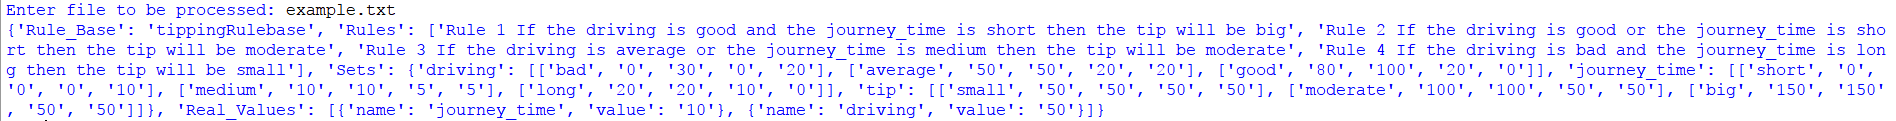
\includegraphics[width=12cm]{example1}
\caption{File Reader example output}
\end{figure}

\subsection{Membership Calculator}
The individual membership calculator module can be found in ‘MembershipCalculator.py’. When executing the file the script will ask the user for the a, b, alpha, beta and value to generate the membership value and return it to the user.  

\begin{figure}[H]
\centering
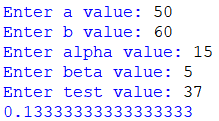
\includegraphics[width=5cm]{example2}
\caption{Membership Calculator example output}
\end{figure}

\subsection{Rule Reader}
The individual rule reader module can be found in ‘RuleReader.py’. When executing the file the script will ask the user for the rule they wish to be read. This rule must follow the pattern indicated in the assignment specification: Rule [x] if the \textless variable\textgreater is \textless value\textgreater [and|or] \textless variable\textgreater is \textless value\textgreater then the will be \textless variable\textgreater \textless value\textgreater. If an input is entered that does not fit this format an error message will be returned. If the input is accepted by the script then it will return a dictionary to the user with the following keys: ID, Variables, Values, Operator, Output. Each key will have it’s corresponding values populated from the relevant section in the inputted rule. 


\begin{figure}[H]
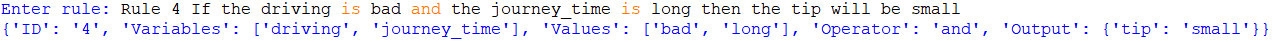
\includegraphics[width=12cm]{example3}
\caption{Rule Reader example output}
\end{figure}

\subsection{Rule Firer}
In order for this module to work, it is necessary that the previous three modules are combined to create a partially complete system. This is required because we need to have a set of rules to work with and we need to be able to calculate membership values. When executing the partial system the script, RuleFirer.py, will ask the user for the name of the file they wish to be used, this is the functionality that was created in the first module, FileReader.py. Within this file should be the rules and variables outlined within the assignment specification in the correct format. The script will use these rules and values to calculate single values for each outcome set. In example.txt the outcome sets are small, moderate and big under the identifier tip.

\begin{figure}[H]
\centering
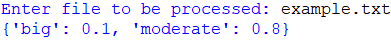
\includegraphics[width=6cm]{example4}
\caption{Rule Firer example output}
\end{figure}

\subsection{Defuzzifier}
Like the rule firer module the defuzzifier can not work without combining the previous four modules together. The defuzzifier requires rules to be fired to defuzz the values returned and the rule firer cannot work without the first three modules. The defuzzifier module can be found in Defuzzifier.py, when executing the file the script will again ask the user for the filename of the file they wish to be used by the script. The defuzzifier will take the values returned from the rule firer module and perform a series of calculations shown  in section \ref{defuzz} to return the final defuzzified value to the user.

\begin{figure}[H]
\centering
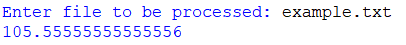
\includegraphics[width=6cm]{example5}
\caption{Defuzzifier example output}
\end{figure}

\section{Testing}
\subsection{File Reader}
\begin{center}
 \begin{tabular}{ |p{2cm}|p{3cm}|p{3cm}|p{3cm}|  }
 \hline
 Test Number & Document Tested & Expected Result & Actual Result \\ [0.5ex] 
 \hline\hline
 1 & example.txt & Dictionary 1 in expectedfile.txt should be returned. & Output matches dictionary 1. \\ 
 \hline
 2 & example2.txt & Dictionary 2 in expectedfile.txt should be returned. & Output matches dictionary 2. \\
 \hline
 3 & errorexample.txt & Script should terminate with no output. & Script terminates. \\
 \hline
 4 & Any filename that does not exist, “empty.txt” for example & Script should terminate with no output. & Script terminates. \\
 \hline
\end{tabular}
\end{center}

\subsection{Membership Calculator}
To perform this test I will use the following 4 tuple:  Middle-Age (50,60,15,5) with the following ages: 20,37,55,63,85
\begin{center}
 \begin{tabular}{ |p{2cm}|p{3cm}|p{3cm}|p{3cm}|  }
 \hline
 Test Number & Inputs & Expected Result & Actual Result \\ [0.5ex] 
 \hline\hline
 1 & 50,60,15,5,20 & 0 & 0 \\ 
 \hline
 2 & 50,60,15,5,37 & 0.13 & 0.13 \\
 \hline
 3 & 50,60,15,5,55 & 1 & 1 \\
 \hline
 4 &50,60,15,5,63 & 0.4 & 0.4 \\
 \hline
 5 & 50,60,15,5,85 & 0 & 0 \\
 \hline
\end{tabular}
\end{center}

\subsection{Rule Reader}
\begin{center}
 \begin{tabular}{ |p{2cm}|p{3cm}|p{3cm}|p{3cm}|  }
 \hline
 Test Number & Document Tested & Expected Result & Actual Result \\ [0.5ex] 
 \hline\hline
 1 & Rule 1 If the driving is good and the journey\textunderscore{time} is short then the tip will be big & \{'ID': '1', 'Variables': ['driving', 'journey\textunderscore{time}'], 'Values': ['good', 'short'], 'Operator': 'and', 'Output': \{'tip': 'big'\}\}  &  \{'ID': '1', 'Variables': ['driving', 'journey\textunderscore{time}'], 'Values': ['good', 'short'], 'Operator': 'and', 'Output': \{'tip': 'big'\}\}  \\ 
 \hline
 2 & Rule1 If the driving is good and the journey\textunderscore{time} is short then the tip will be big & Invalid Rule & Invalid Rule \\
 \hline
 3 & Empty String & Invalid Rule & Invalid Rule \\
 \hline
 4 & rule 4 if the temperature is low and the current is low then the result will be increaseCurrent & \{'ID': '4', 'Variables': ['temperature', 'current'], 'Values': ['low', 'low'], 'Operator': 'and', 'Output': \{'result': 'increaseCurrent'\}\} & \{'ID': '4', 'Variables': ['temperature', 'current'], 'Values': ['low', 'low'], 'Operator': 'and', 'Output': \{'result': 'increaseCurrent'\}\} \\
 \hline
 5 & Rule 4 If driving is bad and the journey\textunderscore{time} is long then the tip is small & Invalid Rule & Invalid Rule \\
 \hline
\end{tabular}
\end{center}


\subsection{Rule Firer}
\begin{center}
 \begin{tabular}{ |p{2cm}|p{3cm}|p{3cm}|p{3cm}|  }
 \hline
 Test Number & Document Tested & Expected Result & Actual Result \\ [0.5ex] 
 \hline\hline
 1 & example.txt & Big = 0.1\newline Moderate = 0.8 & Big = 0.1\newline Moderate = 0.8 \\ 
 \hline
 2 & example2.txt & Reduce Current = 0.7\newline No Change = 0.3 & Reduce Current = 0.7\newline No Change = 0.3 \\
 \hline
 3 & errorexample.txt & Script should terminate with no output. & Script terminates. \\
 \hline
 4 & Any filename that does not exist, “empty.txt” for example & Script should terminate with no output. & Script terminates. \\
 \hline
\end{tabular}
\end{center}


\subsection{Defuzzifier}
\begin{center}
 \begin{tabular}{ |p{2cm}|p{3cm}|p{3cm}|p{3cm}|  }
 \hline
 Test Number & Document Tested & Expected Result & Actual Result \\ [0.5ex] 
 \hline\hline
 1 & example.txt & 65 & 65 \\ 
 \hline
 2 & example2.txt & Reduce Current = 0.7 \newline No Change = 0.3 & Reduce Current = 0.7, No Change = 0.3 \\
 \hline
 3 & errorexample.txt & Script should terminate with no output. & Script terminates. \\
 \hline
 4 & Any filename that does not exist, “empty.txt” for example & Script should terminate with no output. & Script terminates. \\
 \hline
\end{tabular}
\end{center}
The only difference here between expected and actual results is the accuracy of the floating point number in test number 1. The system returns a more accurate number so there is no problem with the mismatch.

\subsection{Full System}
To exhaustively test the full system’s reliability, I will use the rule base found in example.txt and change the real world values to ensure the correct results are returned in different circumstances. As a general rule, tests where driving is good and journey times are short should always return a higher value than those that represent the opposite. The first few tests will be based on the more extreme scenarios and then the rest will deviate slightly to see how the output value changes. If the journey time increases the tip should be less and vice versa. If the driving quality increases the tip should also increase and vice versa. There are also instances where given the real world values where the rule firing will only return one potential membership, in this example \{small:1\}. If given this value, the system will return the maximum value of that tuple in the rule base. For this test set, those max values are 50 for small, 100 for moderate and 150 for big.

\begin{center}
 \begin{tabular}{ |p{2cm}|p{4cm}|p{3cm}|  }
 \hline
 Test Number & Real World Values & Result \\ [0.5ex] 
 \hline\hline
 1 & journey\textunderscore{time} = 9  \newline driving = 65 & 105.55555555555556  \\ 
 \hline
 2 & journey\textunderscore{time} = 4  \newline driving = 77 \newline (This represents a very good scenario) & 120.6896551724138  \\ 
 \hline
 3 & journey\textunderscore{time} = 19  \newline driving = 10 \newline (This represents a very bad scenario) & 50  \\ 
 \hline
 4 & journey\textunderscore{time} = 12  \newline driving = 35 \newline (This represents a very average scenario) & 87.5  \\ 
 \hline
 5 & journey\textunderscore{time} = 6  \newline driving = 80 & 114.28571428571429  \\ 
 \hline
 6 & journey\textunderscore{time} = 8  \newline driving = 80 & 108.33333333333333  \\ 
 \hline
 7 & journey\textunderscore{time} = 8  \newline driving = 70 & 112.5  \\ 
 \hline
 8 & journey\textunderscore{time} = 5  \newline driving = 100 & 125  \\ 
 \hline
 9 & journey\textunderscore{time} = 20  \newline driving = 20 & 50  \\ 
 \hline
 10 & journey\textunderscore{time} = 10  \newline driving = 50 & 100  \\ 
 \hline
\end{tabular}
\end{center}

As can be seen the system behaves as one would expect from a Fuzzy Logic system, as the real world values change the tip either increase or decreases as would be expected given the rules within the rule base.

\section{Evalulation}
\subsection{Limitations}
\begin{itemize}
  \item Rulebase must follow the layout outlined in the specification strictly.
  \item If there is an issue within the rulebase file the system will terminate abruptly.
  \item Rules must follow a strict pattern.
  \item Only one type of conditional operator may be used within a single rule.
  \item A single rule can only have one conditional operator.
\end{itemize}
\subsection{Future Work}
\begin{itemize}
  \item Improve user interface and add visualisation of the data.
  \item Improve error catching.
  \item Allow for flexibility in rulebase and rule formatting.
\end{itemize}

\subsection{Conclusion}
In conclusion, given correctly formatted inputs the system returns a calculated defuzzified output which is fairly accurate, there can be a small margin of difference between values the system returns and hand calculated values bu the margin is never too large for this to become an issue. This is also somewhat to be expected as it is in the nature of fuzzy logic to not have a "fixed" defuzzified value.

\appendix
\section{How to Execute}
This Fuzzy Logic system was implemented using Python version 3.6.1. To run the full system or any of the individual components ensure you have Python version 3 installed on your machine and open a terminal in the directory containing the python files. To run the desired file type: python {filename}.py. Below is an example of the output you should receive if the Full System is executed.
\begin{figure}[H]
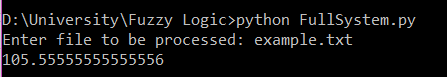
\includegraphics[width=12cm]{manual1}
\caption{Command Line Execution}
\end{figure}
Alternatively the python file can be opened in IDLE and run from there by pressing F5 or selecting Run from the taskbar.
\begin{figure}[H]
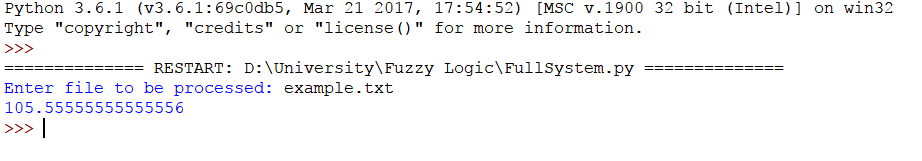
\includegraphics[width=12cm]{manual2}
\caption{Python Shell Execution}
\end{figure}
\end{document}

